We provide two examples here for illustration and evaluation of our Coq plugin. 

\subsection{Type Safety for STLC}\EDJ{We need a fuller view of the two examples. Especially show "accessing family components outside that family".}

\begin{wrapfigure}{r}{0.5\textwidth}\YZ{It is more convincing if you have four or five family mixin together, positive product, negative product, sum type, boolean, and natural number, general recursion and one more}
\begin{lstlisting}[language=Coq,frame = single, escapeinside={@}{@}]
Family STLC_prod.
 Extend FInductive ty : Set :=
  | ty_prod : ty -> ty -> ty.
 Extend FInductive tm : Set :=
  | tm_prod : tm -> tm -> tm  
  | tm_pi1 : tm -> tm  
  | tm_pi2 : tm -> tm.
 Extend Family subst_internal.
  Final Field tm_prod := ..
  Final Field tm_pi1 := ..
  Final Field tm_pi2 := ..
 EndFamily.

 Inherits subst.
 ...
 Extend FInductive has_type 
  : context -> term -> type := ...
 Extend FTheorem subst_lemma.
  ... 
 Qed.
(* ... and more, end with type safety *)
(* Next, Invoking Mixin Command *)
EndFamily.
Family STLC_bool_prod 
    extends STLC 
    using STLC_bool using STLC_prod.
\end{lstlisting}
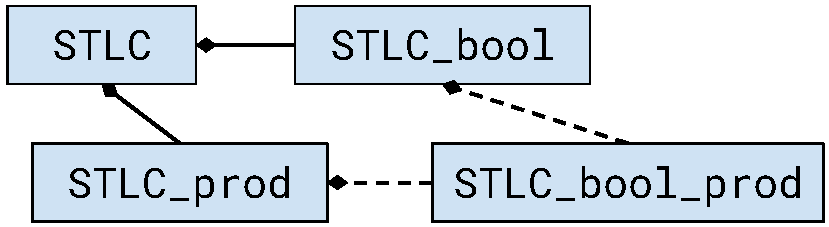
\includegraphics[width=0.5\textwidth]{coqexmaple/STLC-inheritances.pdf}
\caption{Example STLC extended with product, and Mixin with \cref{fig:STLC-example2}}
\end{wrapfigure}

We start with the very basic type safety proof of STLC, largely adapted
from Software Foundation~\cite{pierce2014software}, which is also one of
the primal motivating example of this project. 


Our emphasis here is that, we singled out some language features from
STLC and prove the type safety for each feature separately, following
the style of the examples in MTC~\cite{delaware2013,forsta2020}.
And we use a \textit{not-yet-formally-defined} \textbf{mixin} feature
to mix the semantics and properties of two language features---product
and boolean (in \cref{fig:STLC-example})---with vanilla STLC.

\textbf{Mixin} is implemented by making inheritance judgement/data supporting \textit{weakening} and composition. Then, using notation from metatheory, given $\goodInh{\cdot}{i_1}{\sigma_1}{\sigma_2}$ and $\goodInh{\cdot}{i_2}{\sigma_1}{\sigma_3}$, we can weaken $i_2$ to $\goodInh{\cdot}{i_2'}{\sigma_2}{\sigma_3'}$ and the composition of $i_1$ and $i_2'$ is the resulting mixin---this implementation breaks commutativity and will need to solve design problems on compatibility (mostly related to the \textit{diamond problem}): for example, when $i_1$ and $i_2$ are both extending with a field of the same name, do we signal error or use $i_2$'s extension and consider it as an `override'? However, our current example of STLC only uses a subset of the mixin with a clear semantic (i.e. every sensible design of mixin should agree on)---because our STLC examples only use extension of fields with different names and no overriding is used. 

Note that, every top level family can be considered as an inheritance because (1) our implementation is simplified by considering every family as an inheritance, and (2) we want to align with the complete family polymorphism advocated by \citet{zm2017} where the user can override the parent of the inheriting family (inside a family due to late-binding), and in these case the nested inheriting family is more a inheritance data than a ``standalone'' linkage. Thus we will store for every top level family in our plugin the corresponding inheritance data together with a ``reference'' to the parent family. Then our mixin command can single out the inheritance data from "STLC_bool" and "STLC_prod" and ``mixin'' the inheritance to reach "STLC_bool_prod". 

Using this example,
we hope one day we can say precisely, \textit{a programming language feature itself is a
piece of data/inheritance judgement/inherited family}. Compared with MTC,
our example uses small-step operational semantics\YZ{Does MTC not define a small-step operational semantics for STLC?}\EDJreply{I thought they use big step with fuel. Though Coq a la carte use small-step in one example} by exploiting
extensible inductive types. 

Most of the proof and computation are directly adapted
from the one in Software Foundation, resulting in a similarly accessible proof, while the proof for each extended feature are scattered in the extended families resulting better modularity. One kind of examples is about the computation, for example, substitution functions. Substitutions dealing with product and projection are defined in the corresponding children family. This is mainly done by inheriting and extending the handler family from the parents. The other kind of examples are about propositions and we directly use "(Extend) FTheorem" to handle them. In these cases we don't need to additionally define a auxillary handler family like we did for substitution---we simply use "Extend FTheorem" and our plugin will prepare the goals to prove. At the end, it will look like scattered proof scripts in a modular manner.
For example, the proof on progress on product projection is carried out in the children family that extend "tm" with products. \YZ{Can you say more about how your plugin enables more code reuse and modularity?}\EDJreply{please check}
% In related work, Coq/Metatheory a la carte/Tion embedding can be emphasized as a more "semantic approach" because they encode the meaning using a special design pattern (for example, open recursive inductive type for extension), compared to our more syntactic approach. Their advantage is the transferability of this technique accross different proof assistants, and their disadvantage is that their approach are less accessible and unfriendly to amateur Coq users---which can be reflected from the distance of their approach and text-book Software Foundation proof. 

% We have problem on inversion lemma. Check if it is the same problem as MTC
We use "Closing Fact" to state and prove the inversion lemma instead of
using the extensible proving mechanism "FTheorem". The reasons are that
(1) it introduces much less boilerplate code because the proof for these
inversion lemmas should be just simple case analysis and we should rely
on Coq to generate most of the boilerplate code;\YZ{I was under the impression that the plugin could not auto-generate Closing Facts or their proofs, no?}\EDJreply{I have make the above Closing Fact section more about this detail. Please check.} (2) it shouldn't bother us in the future
because any extension on the syntax should still satisfy these inversion
lemmas; (3) most importantly, we believe this inversion ``lemma'' should
be part of the definition of the syntax instead of considering the
syntax as a mere concrete inductive type. We should postulate this
inversion ``lemma'' like \textit{a constraint} and post-hoc-ly verify
that our inductive definition does satisfy the constraint, which is
exactly what we expect from "Closing Fact". If directly working on inductive definition doesn't bring us benefit during proof engineering, then decompose the property (the constraint) with the concrete definition might be a good idea.

Our formulation for bare STLC is around 400+ LOCs; the two families implementing product and boolean features both take around 250+ LOCs. 
% need comparison with the original implementation

The biggest difference in the proof script comes from the fact that we
are handling ``extensible'' inductive types instead of real inductive
types, and thus the inversion tactic is not working and we have to manually
create inversion lemmas. 

Another difference comes from the fact that we need to use "Closing
Fact" to manually verify the computational rules for each recursor and
use tactics to ``run'' the recursor by repeatedly "rewrite" using those
verified computational rules. This part is possible to be automatically
generated by the plugin, but still it will require propositional 
computational rules.  What's more, we don't yet support the \mintinline{Coq}{Hint}. These three differences on experience lead to a mild code bloat. 

\subsection{Abstract Interpreters for \texttt{Imp}}\YZ{Try to have two runnable interpreter -- choose another simple one like constant propagation. and remove LangMore}
The second example is adapted and modified from \citet{zm2017}.
Contrary to our first example, here, we use a big-step interpreter with fuel
as the operational semantics of an imperative language with
side effects, and we specify the abstract interpretation and prove its
soundness, with some postulation on both computation and property.
Then we extend the base language with new features, and we instantiate
the postulation on computation for
abstract interpreters.
Thanks to the compilation to Coq module, we can directly run the resulting
abstract interpreters.

\begin{figure}[!htb]
  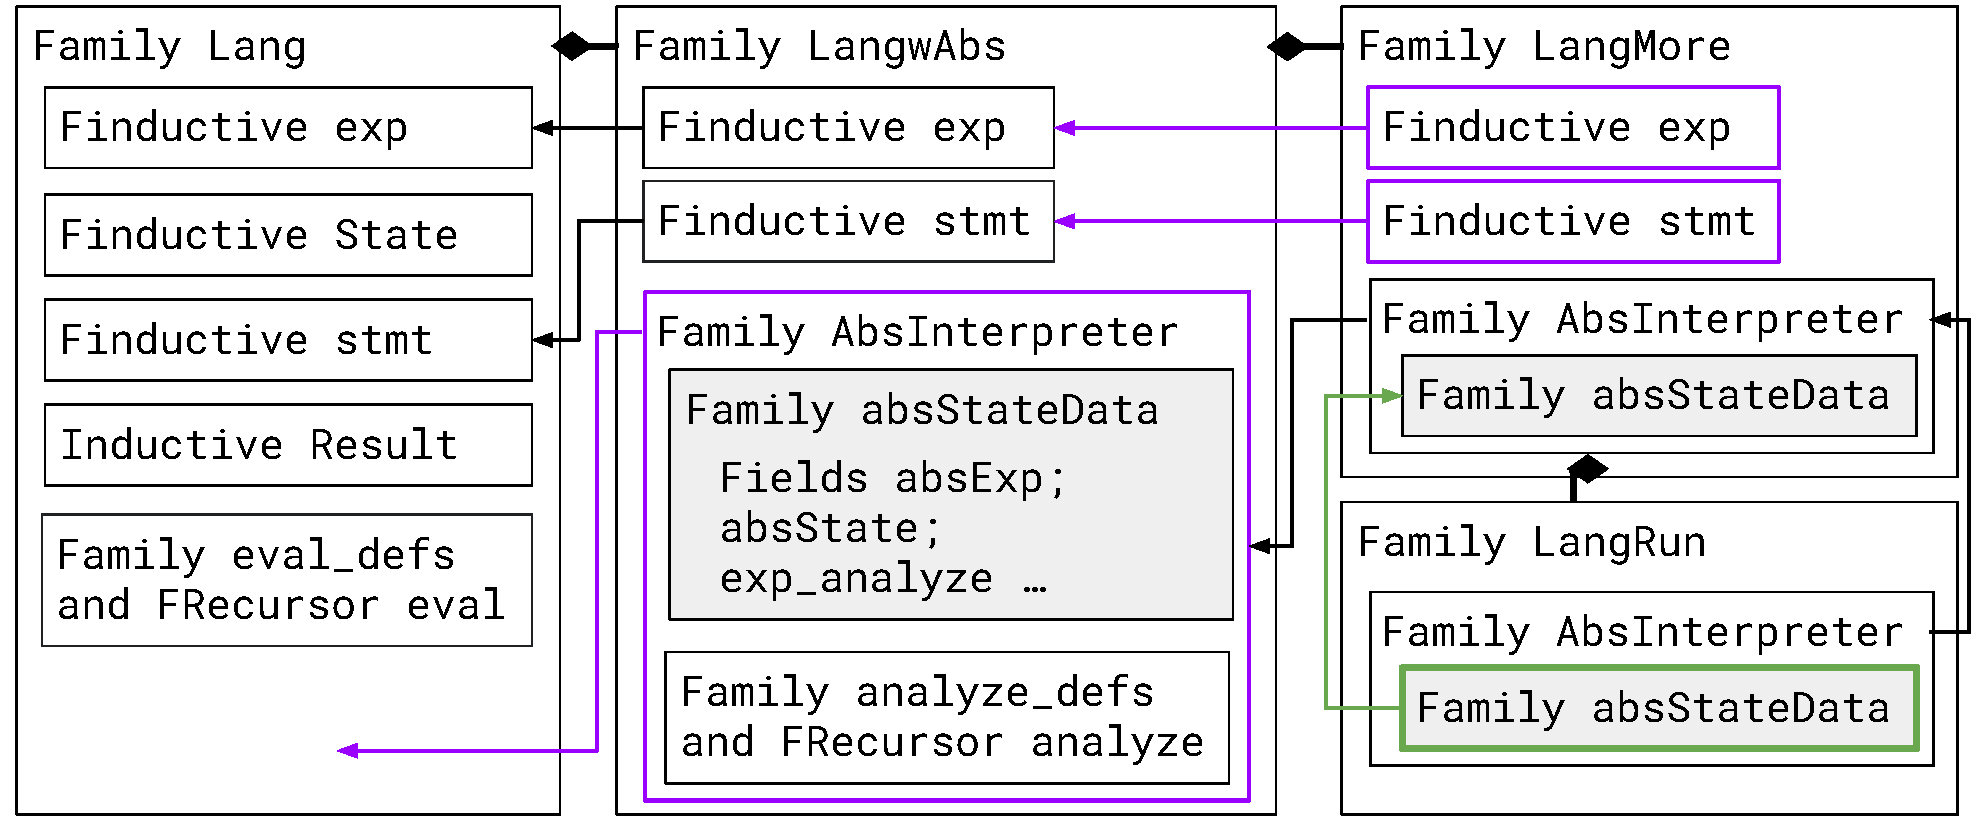
\includegraphics[width=\columnwidth]{coqexmaple/Family-Lang-Imp2.pdf}
  \caption{Inheritance Diagram for Abstract Interpretation Example. Black arrows are inheritance. Purple arrow are extending. Green arrows are overriding. Grey box are sealed families.}\label{fig:abstract-interpretation-example}
\end{figure}

We construct four families, in one inheritance chain, illustrated in \cref{fig:abstract-interpretation-example}.\YZ{Why is it useful to define these concrete and abstract interpreters as an inheritance chain?}\EDJreply{I don't think these examples are here to show the example themselves are useful. They are here to show family inheritance is useful, and can extend stuff to all sorts of things. I also add some details below on how each family can be extended and what each family means.}\YZreply{Why is it desired to define the abstract interpreter as an extension of the concrete interpreter family? What is lost by putting the two interpreters in the same family?}\EDJreply{Nothing is lost. This is just simulating people starting with bare (big-step) operational semantic. Because they may not working on abstract interpretation from the first place. Those people may extend "Lang" with other stuff like another type-safety proof or something.}


The first family "Lang" define the big step operator (using fuel) of a
while language, with expression and stmt defined upon expression. Final "Result" can be error, "out-of-fuel" or a legitmate "State". It takes about 200+ LOCs. 
% We
% can
\YZ{In general, in a result section like this, you want to show what
you *have done* rather than what you *can do*.}\EDJreply{Ok. deleted. I initially want to emphasize ``I **can** use arbitrary implementation for this environment mapping interface'' but I don't know how to say that without using ``can''.}
% swap the implementation of "State" to have different memory/state
% management by extending family "Lang".
\YZ{What is 'different
memory/state management'?}\EDJreply{Actually I should say environment mapping/dictionary. I instantiate it with function(closure) as environment mapping in "LangRun". It is possible to use other mapping like Coq's primitive dictionary.}

The second family "LangwAbs" define the abstract interpreter for "Lang" in "LangwAbs.AbsInterpreter",
together with a bunch of postulates as a big sealed family "absStateData". Then we prove the correctness of the
abstract interpretation function "analyze". It takes about 300+ LOCs. This example shows how
to use family inheritance to extend a concrete interpreter with abstract
interpreters. 
% This example also shows in this family polymoprhism framework we can reason about "Lang" with computation details being abstracted. 

The third Family "LangMore" extend "LangwAbs" with nat constant and
addition, and if-then-else control flow, of course retaining all the
soundness theorem. It takes about 200+ LOCs. This is one example of
using family inheritance to support new language feature, and compatible
with the existent reasoning in "LangwAbs.AbsInterpreter". 

The fourth family "LangRun" instantiate some of the postulates of the
"LangMore" and recover computational information of "analyze". The "absStateData" is overridden by a concrete definition. The resulting abstract interpreter is expected
to act as a type-analyzer. It takes about 200+ LOCs. This is one example
of instantiate the detail computation of abstract interpretation. 


And at the end, we compile LangRun into module and use Coq to run it on
some simple queries. This "LangRun" also illustrates that we still have
computability in the presence of family.\YZ{Can there be a diagram (a la Figure 1 in Familia paper) illustrating the relationships between (and functionalities of) the different families?}\EDJreply{Done. Please check}

